\part{Introduction}
\begin{frame}
\partpage
\end{frame}

\begin{frame}{Health and Safety}
\begin{columns}[c]
\begin{column}{0.33\textwidth}
\begin{center}

\includegraphics[width=0.8\textwidth,height=0.5\textheight,keepaspectratio]{imgs/health-safety-1.png}\\

\includegraphics[width=0.8\textwidth,height=0.5\textheight,keepaspectratio]{imgs/health-safety-4.png}
\end{center}
\end{column}
\begin{column}{0.33\textwidth}
\begin{center}

\includegraphics[width=0.8\textwidth,height=0.5\textheight,keepaspectratio]{imgs/health-safety-2.png}\\
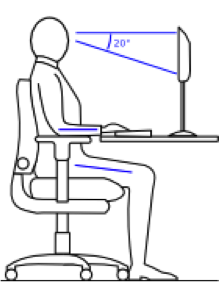
\includegraphics[width=0.8\textwidth,height=0.5\textheight,keepaspectratio]{imgs/health-safety-5.png}
\end{center}
\end{column}
\begin{column}{0.33\textwidth}
\begin{center}

\includegraphics[width=0.8\textwidth,height=0.5\textheight,keepaspectratio]{imgs/health-safety-3.png}\\

\includegraphics[width=0.8\textwidth,height=0.5\textheight,keepaspectratio]{imgs/health-safety-6.png}
\end{center}
\end{column}
\end{columns}
\end{frame}

\section{Who are we?}
\begin{frame}{UIS: Research and Institutional Services Division}
Your trainers for today will be:\\
\begin{itemize}
  \item Paul Sumption --- Research Computing Technical Liaison
    \item Mark Sharpley --- Computer Officer, WT/MRC Stem Cell Institute
  \item\alert{Please ask questions and let us know if you need assistance.}
\end{itemize}
\end{frame}

\section{More about your trainers}
\begin{frame}{Paul Sumption}
\begin{itemize}
  \item Advising users on Research Computing Services run by UIS
  \item Part of the Research Computing Team
  \item Experienced Linux sysadmin 
  \item Trainer for the introduction to HPC (High Performance Computing) course
  \item\alert{The HPC course is running tomorrow, raise your hand if you are on it!}
\end{itemize}
\end{frame}

\section{More about your trainers}
\begin{frame}{Mark Sharpley}
\begin{itemize}
  \item Computer Officer in the School of Biological Sciences
  \item Linux sysadmin 
  \item Building servers and run a small compute cluster 
\end{itemize}
\end{frame}

\section{Material Pt 1}
\begin{frame}{Introduction: Course Material}
\begin{itemize}
\item Today's course uses a modified version of material that was written for UIS MCS Linux
\item UIS MCS facilities: \url{https://help.uis.cam.ac.uk/service/devices-networks-printing/managed-desktops/mcs/mcr-rooms} 
\item Details of the MCS Linux service: \url{https://help.uis.cam.ac.uk/service/devices-networks-printing/managed-desktops/mcs/basiclinux} 
\end{itemize}
\end{frame}

\section{Material Pt 2}
\begin{frame}{Introduction: Material}
The course has been designed as 'self paced':
\begin{itemize}
\item a) Obtain an MCS account, download the course and then start teaching yourself using a MCS Linux PC and the notes
\item b) Book a place on a UIS course. There is an instructor present to help you if you get stuck on the exercises
\item Our course is being delivered at the Bioinformatics Training Facility
\item We have made quite a few changes to the original material
\item We have tested the exercises but please let us know if you find a mistake in the material 
\end{itemize}
\end{frame}

\section{Introduction: Other Linux Courses}
\begin{frame}{Other Courses}
\begin{itemize}
\item Unix: Introduction to the Command Line Interface (Self-paced)
\small {\url{https://www.training.cam.ac.uk/ucs/Course/ucs-unixintro1}} 
\item{The course that runs on MCS Linux}
\pause
\item Shell scripting:
\item Unix: Simple Shell Scripting for Scientists
\small {\url{https://www.training.cam.ac.uk/ucs/Course/ucs-scriptsci}} 
\end{itemize}
\end{frame}

\section{Introduction: Format for today}
\begin{frame}{Format for today}
\begin{itemize}
\item We have split the self paced material into several sections
\item Before each section we will present some slides to introduce the topic
\item You will then have time to attempt the self paced material for the section
\item During self paced work we will assist you, just put your hand up if you are stuck
\item Your instructors can demonstrate exercises as needed
\end{itemize}
\end{frame}

\section{Today's Session}
\begin{frame}{Today's Session}
\begin{itemize}
\item Course material will be displayed on the left and right hand side screen
\item The central screen will display the course notes or demonstrating exercises
\item Your PC will already be booted into Linux 
\end{itemize}
\end{frame}

\section{Usernames and Passwords}
\begin{frame}{Usernames and passwords}
\begin{itemize}
\item Your desktop PC has a local user account 
\item When we get to the remote server exercise we will give you each a username and password for the remote machine
\end{itemize}
\end{frame}

\section{Course Material}
\begin{frame}{Course Material}
\begin{itemize}
\item We will demonstrate how to access the Course Material on your PC
\item You will find a copy of the course material in your home folder
\item There is a PDF of course notes and exercises
\item The folder 'Linux Intro' contains files and folders needed for the exercises
\item There is a zip file 'LinuxIntro.tgz' which will be use during the remote server exercises 
\end{itemize}
\end{frame}

\section{File Management}
\begin{frame}{Files}
\begin{itemize}
\item Click this icon to start the file manager:

\includegraphics{imgs/files.png}
\item This is similar to Explorer on Windows or Finder on a Mac
\end{itemize}
\end{frame}

\section{Home Folder}
\begin{frame}{Home Folder}
\begin{itemize}
\item Click Files
\item A window will open and display your home folder
\item Click on the 'Linux Intro' folder
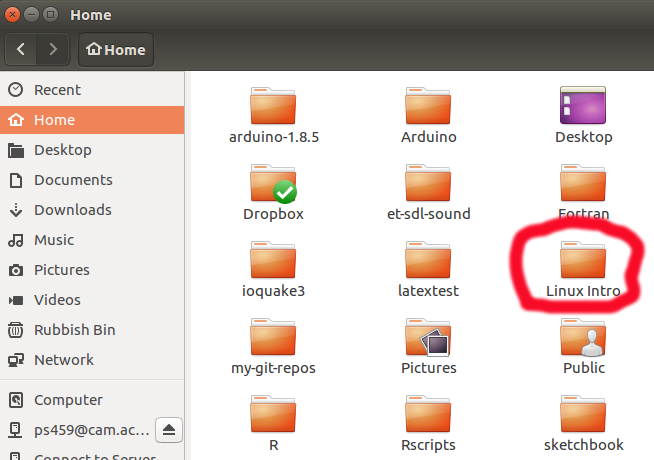
\includegraphics[height=0.5\textheight]{imgs/HomeFolder.png}
\end{itemize}
\end{frame}

\section{Course Folder}
\begin{frame}{Open the Course Folder}
\begin{itemize}
\item Click on the 'Beginners-linux-notes.pdf' folder
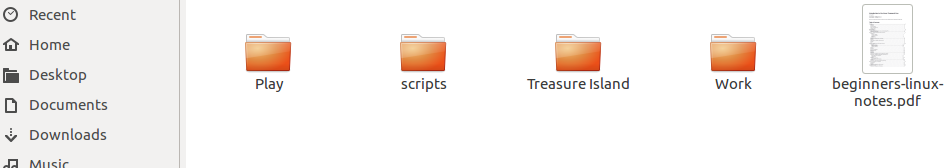
\includegraphics[height=0.2\textheight]{imgs/LinuxIntroFolder.png}
\end{itemize}
\end{frame}

\section{Your Desktop}
\begin{frame}{Your Desktop}
\begin{itemize}
\item Your desktop should look similar to this, notes open, home folder open
\item\alert{Raise your hand if you need help}
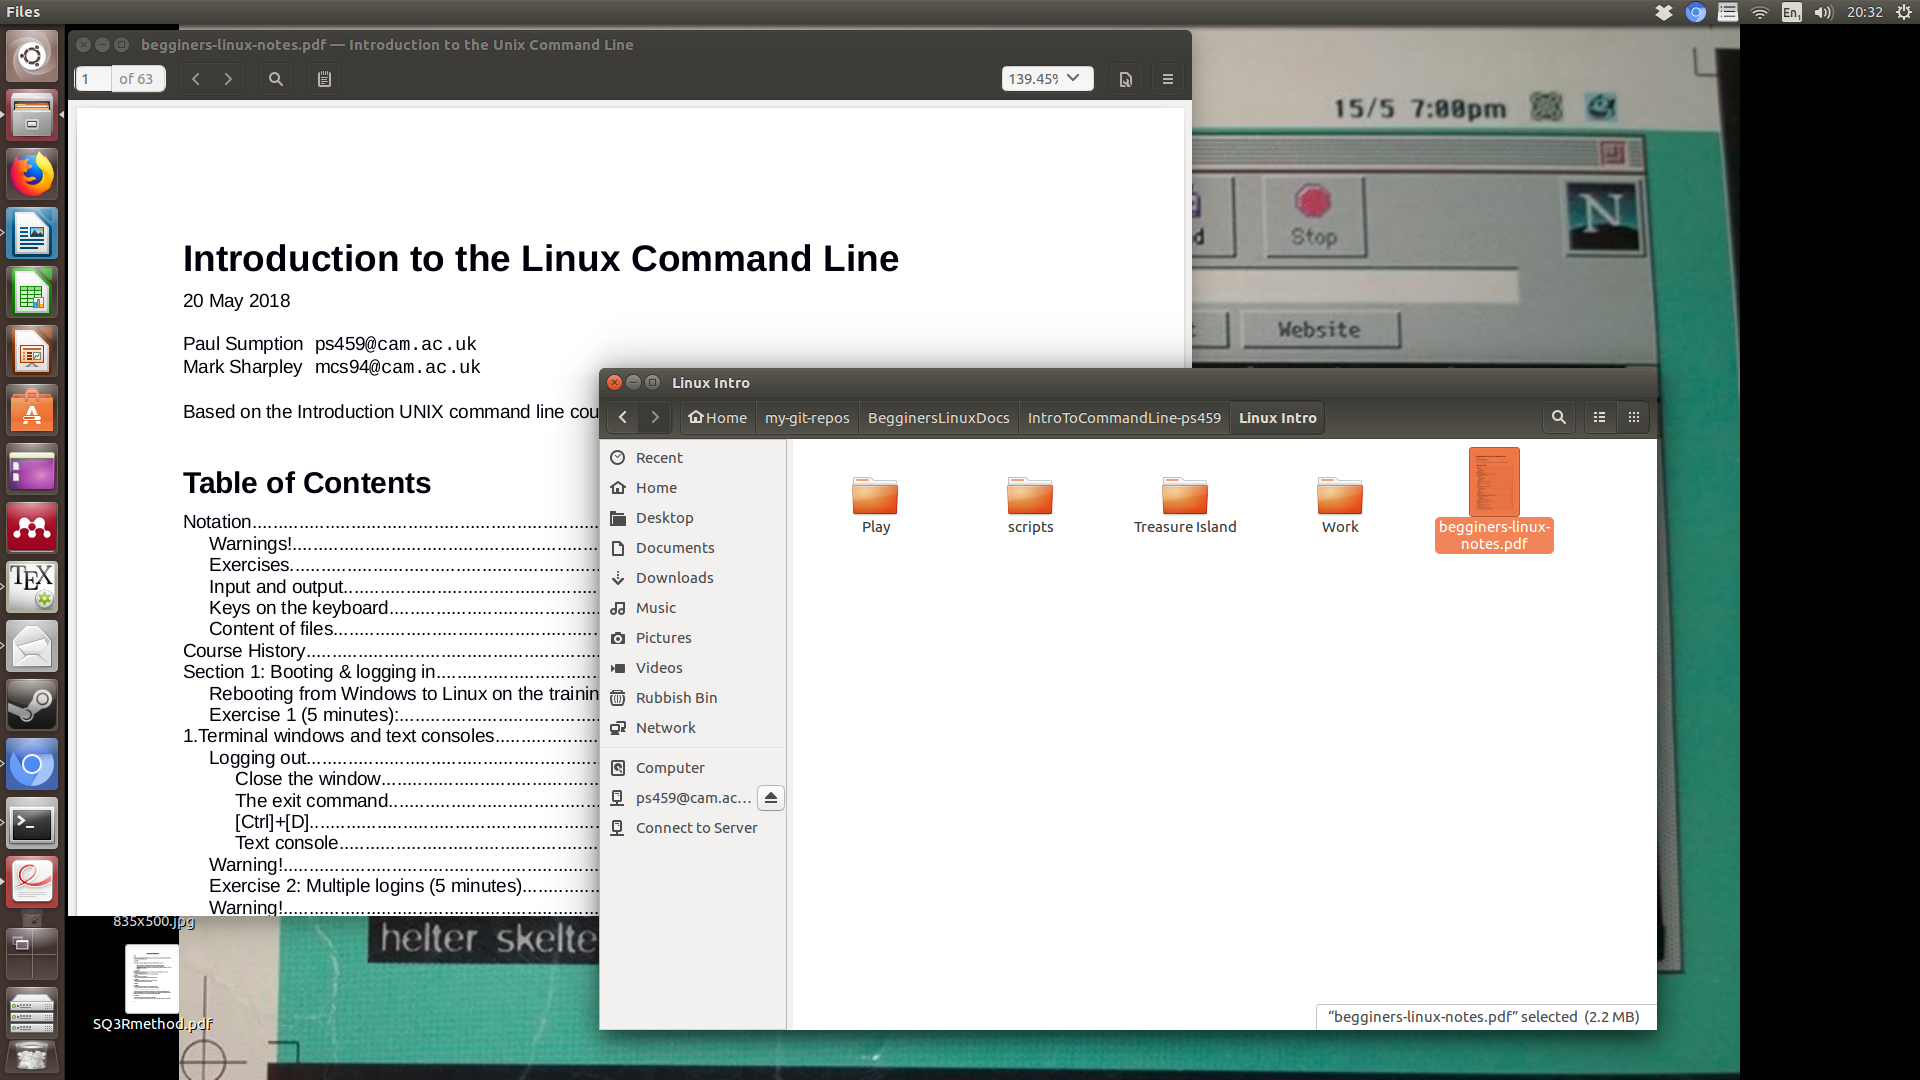
\includegraphics[height=0.5\textheight]{imgs/Desktop.png}
\end{itemize}
\end{frame}




